\documentclass[svgnames,smaller,table]{beamer}
\usepackage{multirow}
\usepackage{tikz}
\usefonttheme[onlymath]{serif}

\usepackage{listings}
% Configura o listings
\lstset{
  %  basicstyle=\footnotesize,\small,...\tiny
  basicstyle=\ttfamily\scriptsize,
  commentstyle=\color{mygreen},
  numbers=left,
  stepnumber=1,
  showstringspaces=false,
  tabsize=2,
  breaklines=true,
  breakatwhitespace=false
 columns=fixed,
 fontadjust=true,
 basewidth=0.5em
}


\usetheme{lthn}
\setbeamercolor*{normal text}{fg=black}
% -----------------------------------------------------------------------------------------------------------------

\title[Slide]{THE LTHN COMPUTER CLUSTER}
%\author{Vitor Vasconcelos Araújo Silva}
\author{Vitor Vasconcelos A. Silva, Graiciany P. Barros, André A. C. dos Santos, Daniel de A. Magalhães Campolina}

\date{\today}
\institute{%
  LTHN - Laboratório de Termo-hidráulica e Neutrônica
  \par
  Serviço de Tecnologia de Reatores - CDTN/CNEN}

\begin{document}

%-------------------------------------------------
\begin{frame}
\titlepage
\end{frame}

%-------------------------------------------------
\begin{frame}
  \frametitle{Outline}
  \tableofcontents%[pausesections]
\end{frame}


\section{Cluster}
%-------------------------------------------------
\subsection{Physical vision}
\begin{frame}
  \frametitle{Cluster}
  \framesubtitle{Meet the beast}
  \includegraphics[scale=0.2]{figuras/duas.jpg}
\end{frame}

\subsection{Schematic vision}
%-------------------------------------------------
\begin{frame}
  \frametitle{Cluster}
  \framesubtitle{Schematic vision of the system}
  \begin{center}
    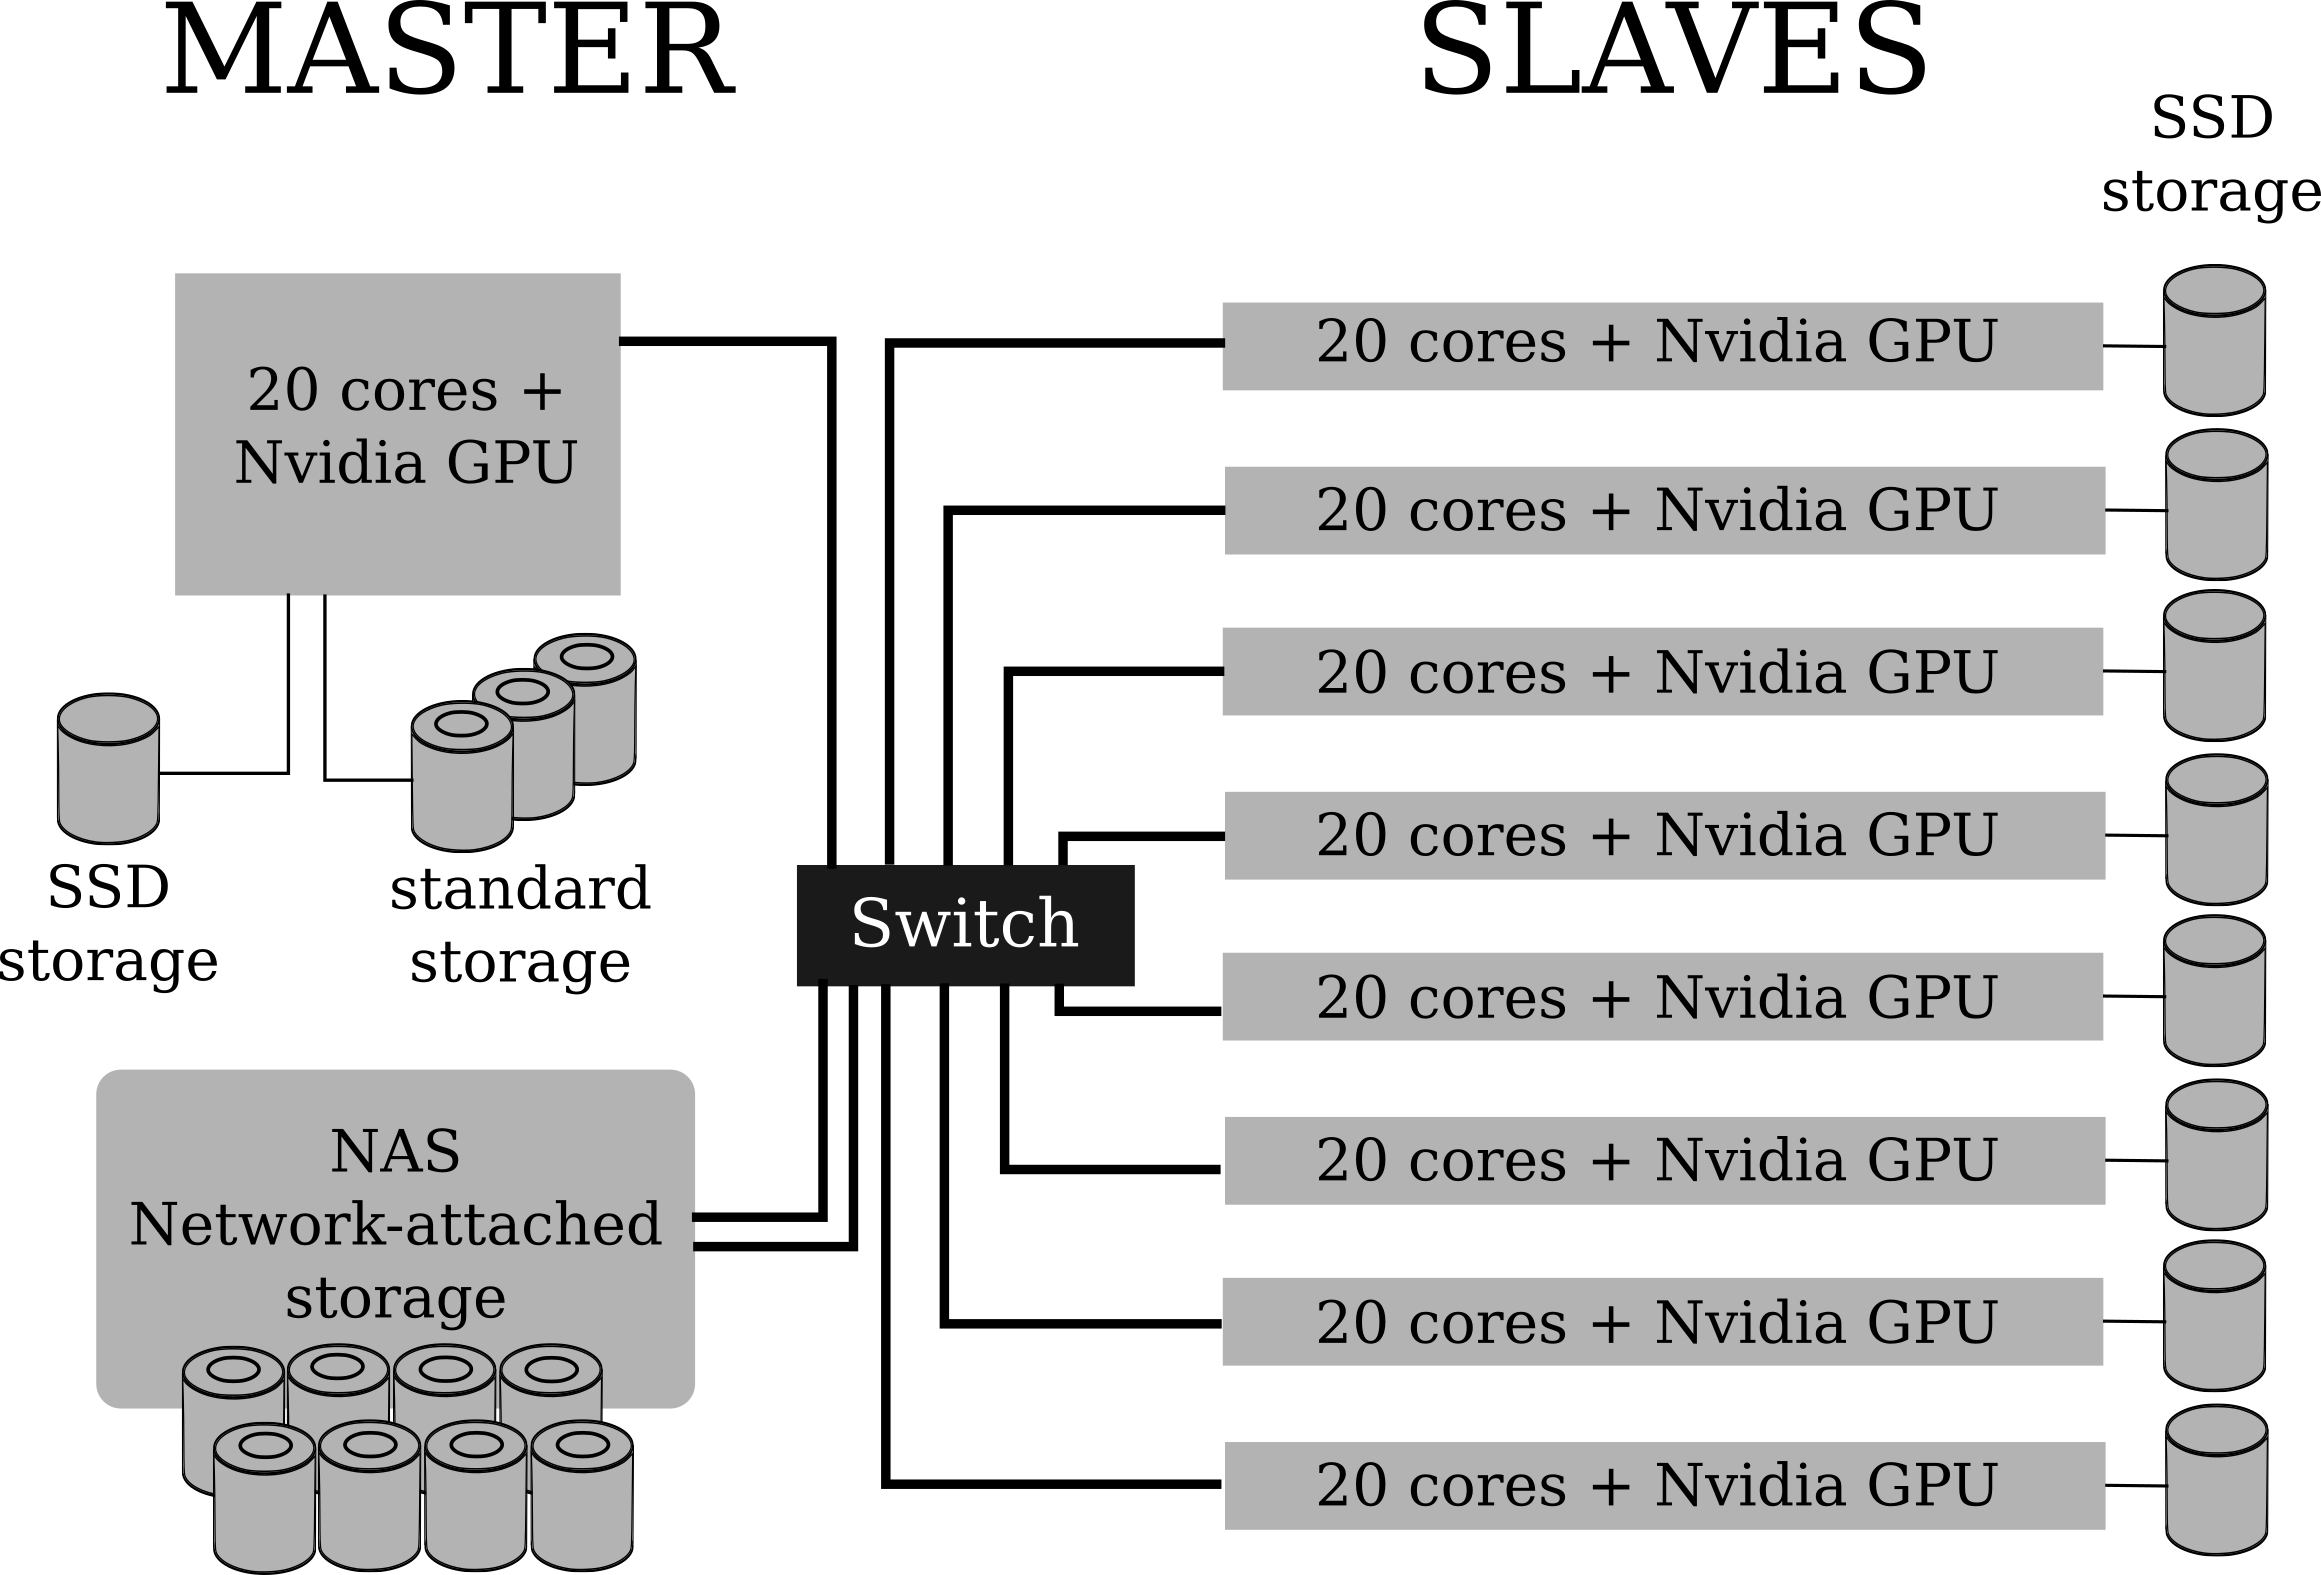
\includegraphics[scale=0.5]{figuras/cluster-topologico.png}
  \end{center}
%  \begin{tikzpicture}[remember picture,overlay]
%    \node[anchor=center, inner sep=0] (img1) at (0,0) {\includegraphics[scale=0.2]{figuras/duas.jpg}};
%    \begin{scope}[
%        x={(img1.south east)},
%        y={(img1.north west)}
%      ]
%      \node [red, font=\bfseries] at (0.25,0.65) {$P(X|Y)$};
%    \end{scope}
%  \end{tikzpicture}
\end{frame}

%-------------------------------------------------
\begin{frame}
  \frametitle{Cluster}
  \framesubtitle{Parts explained}
  \begin{itemize}
  \item \textbf{Master:} The 'head' of the system. This machine is the gateway to the network, the controller of the scheduler system, the host of the webserver, etc.
  \item \textbf{Slaves:} The 'nodes'. These are the heavy duty machines, with only local SDD storage (for OS) and part of the distributed filesystem.
  \item \textbf{NAS:} Network A? System. The secondary computer system which controls the common - cluster and laboratory/institute - data storage devices.
  \item \textbf{Switch:} A high-end network device. This device is responsible for physically connect all parts of the system to allow communication.
  \end{itemize}
  
\end{frame}


\subsection{Characteristics}
%-------------------------------------------------
\begin{frame}
  \frametitle{Cluster}
  \framesubtitle{Characteristics}
  What makes the LTHN cluster so special and differentiate it from a bunch of ordinary computers?\\
  \vspace{10px}
  \begin{itemize}
  \item It uses a \textbf{distributed filesystem}: the files are not contained in one or more physical disks in one machine, but \textbf{all} nodes (and the master) write and read files from any disk of the system. This non-trivial control is made by a special piece of dedicated software (to be mentioned ahead). 
  \item It has a job sheduler system. Its objective is to control the use and schedule the resources, depending on the level of the user and making sure that the system is used at its best. For example, a user requestes a number of processors: the system decide where this processor will be allocated.
  \end{itemize}
\end{frame}

\subsection{Distributed filesystem}

%-------------------------------------------------
\begin{frame}
  \frametitle{Cluster}
  \framesubtitle{Distributed filesystem: works as a \textbf{huge} virtual disk}
    \begin{center}
      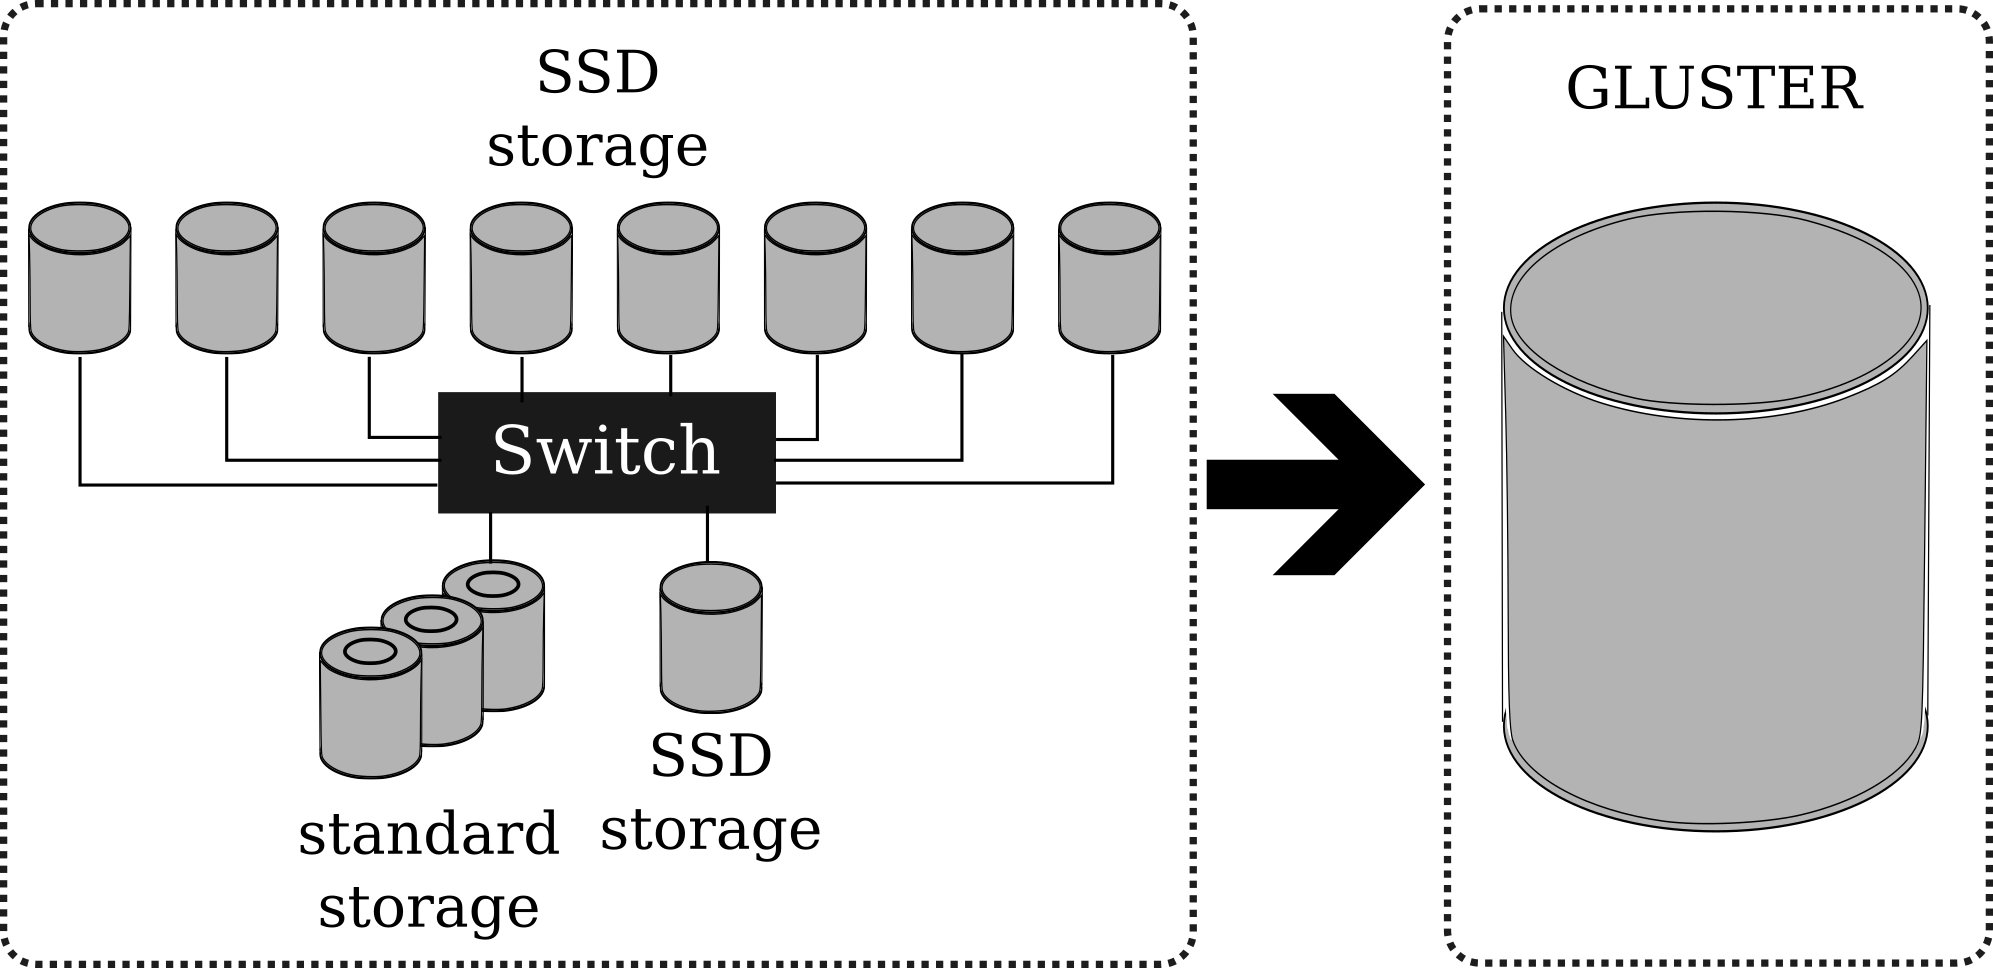
\includegraphics[scale=0.65]{images/gluster.png}
    \end{center}
\end{frame}

%-------------------------------------------------
\begin{frame}
  \frametitle{Cluster}
  \framesubtitle{Distributed filesystem: systems atop of it see all storage space as one unique element.}
    \begin{center}
      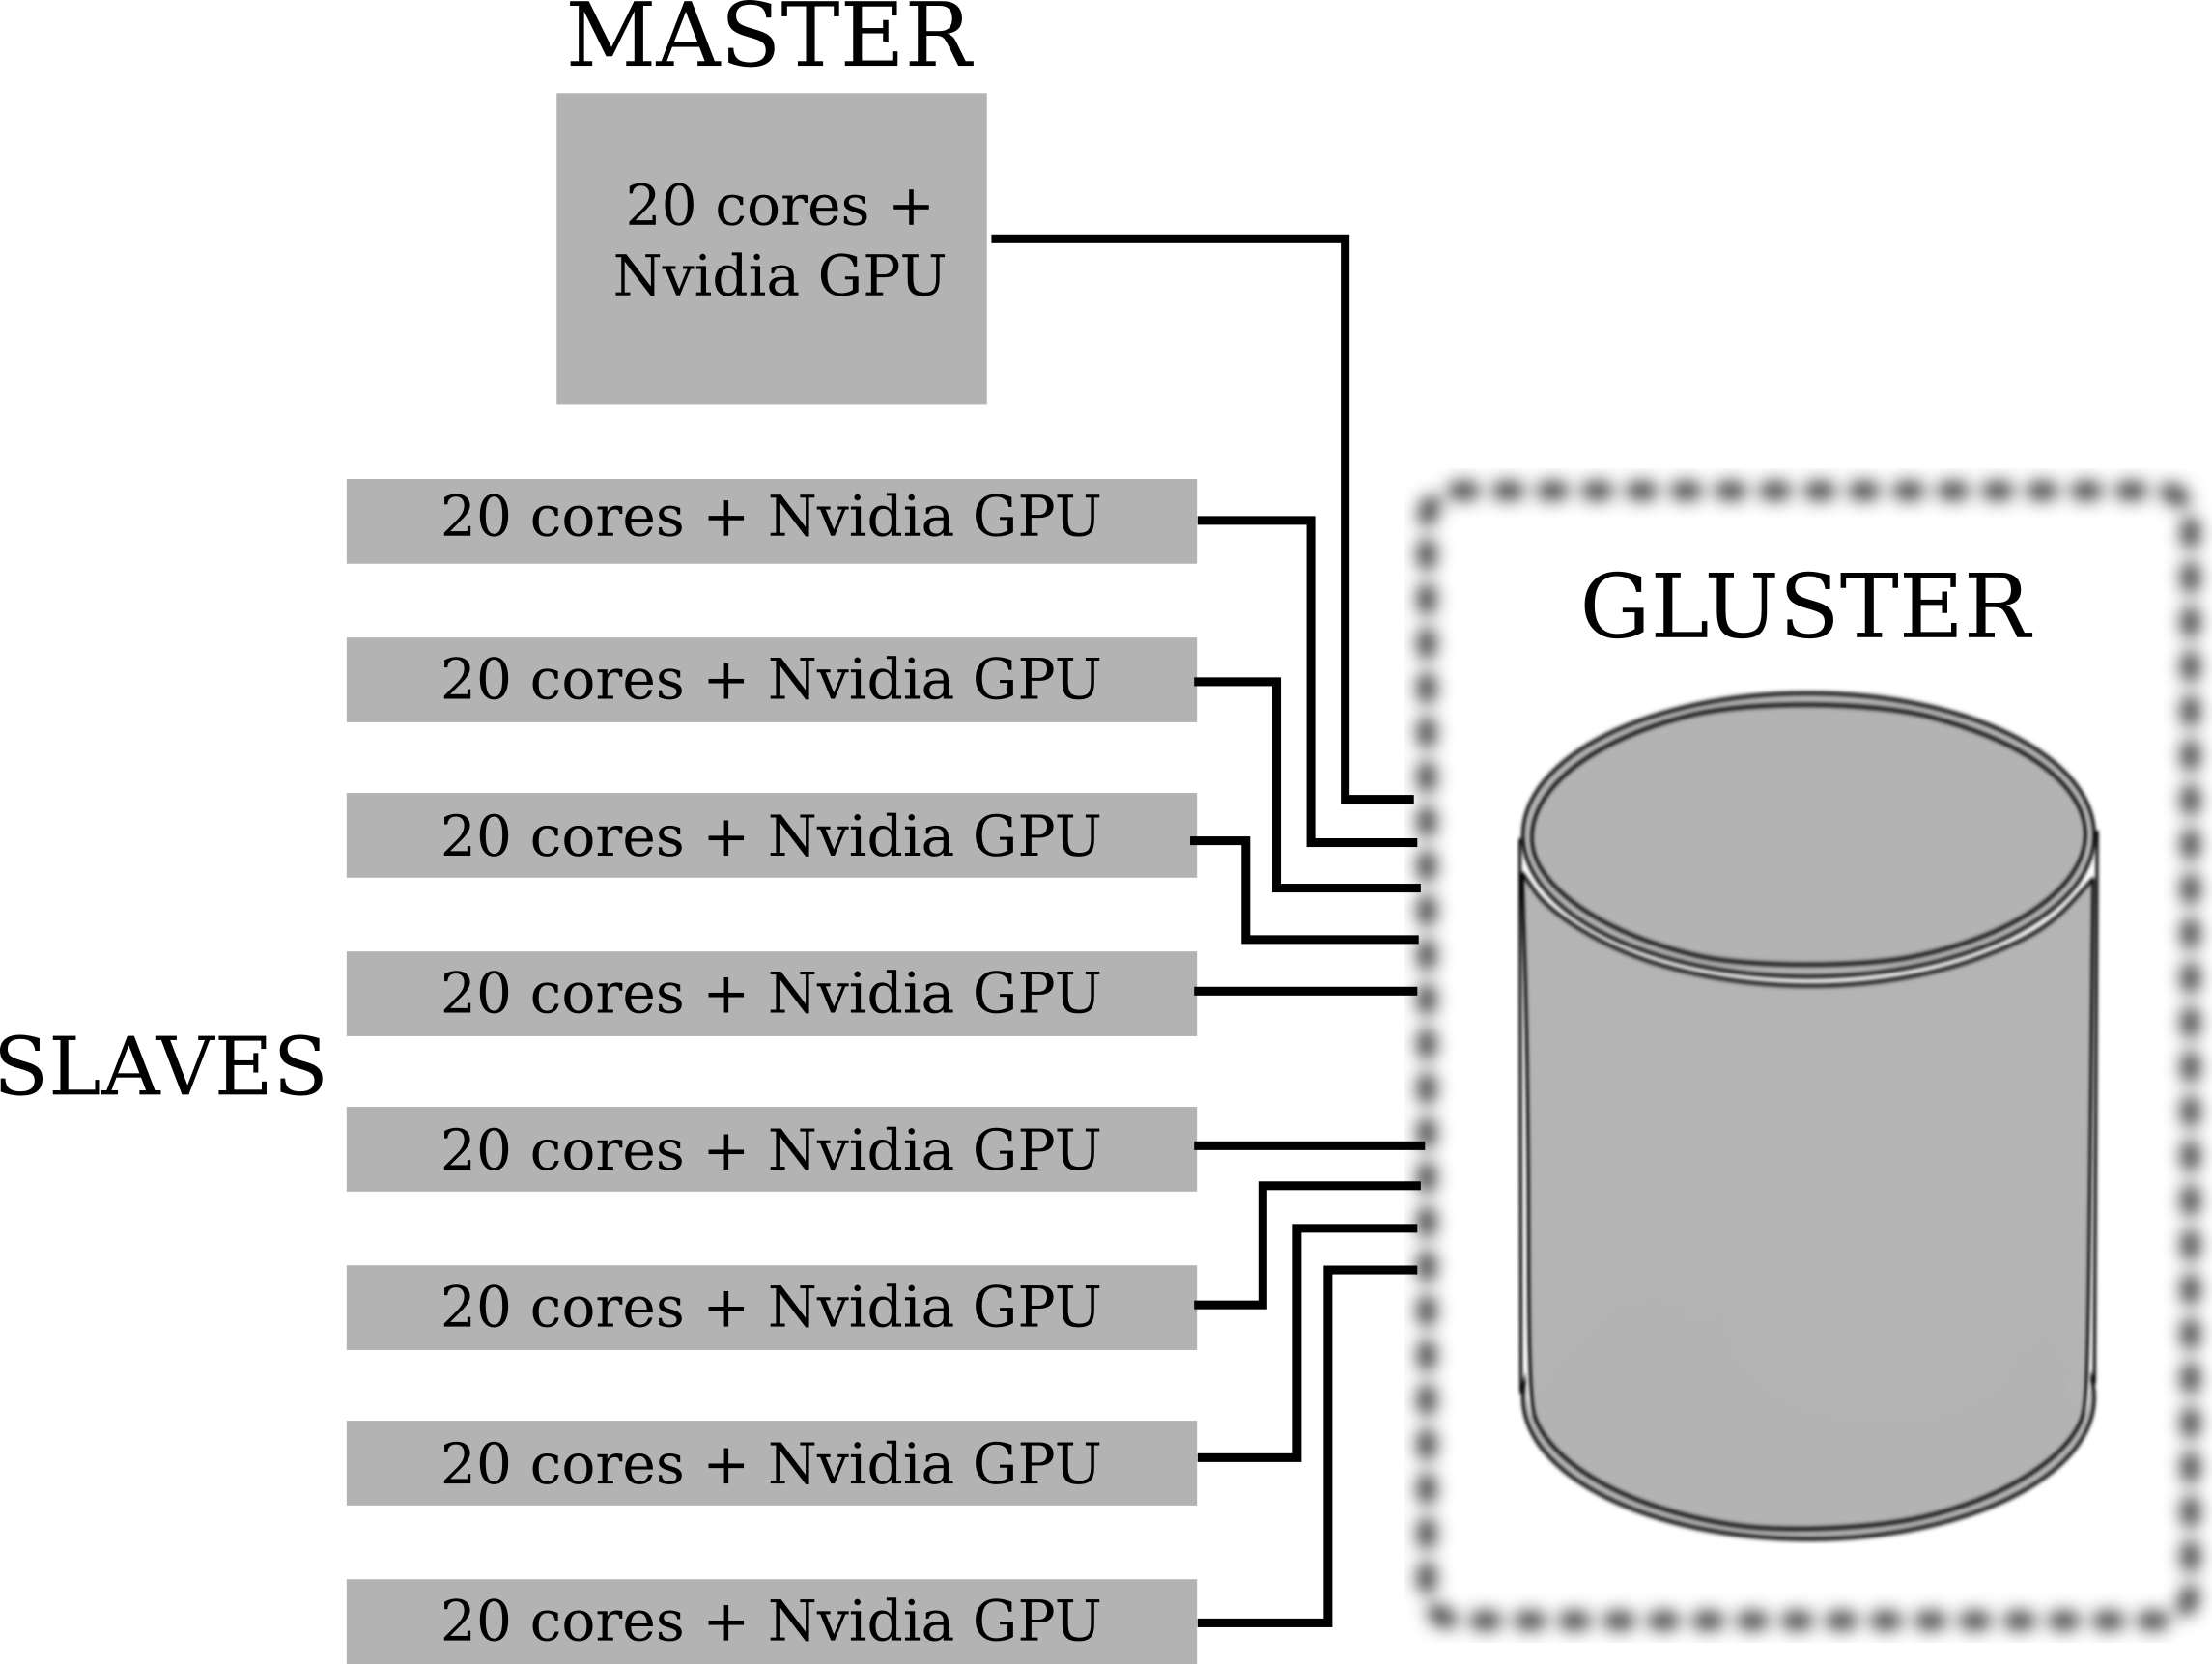
\includegraphics[scale=0.45]{images/cluster-gluster.png}
        \end{center}
\end{frame}

\subsection{Network topology}
%-------------------------------------------------
\begin{frame}
  \frametitle{Cluster}
  \framesubtitle{Network topology}
  \begin{center}
    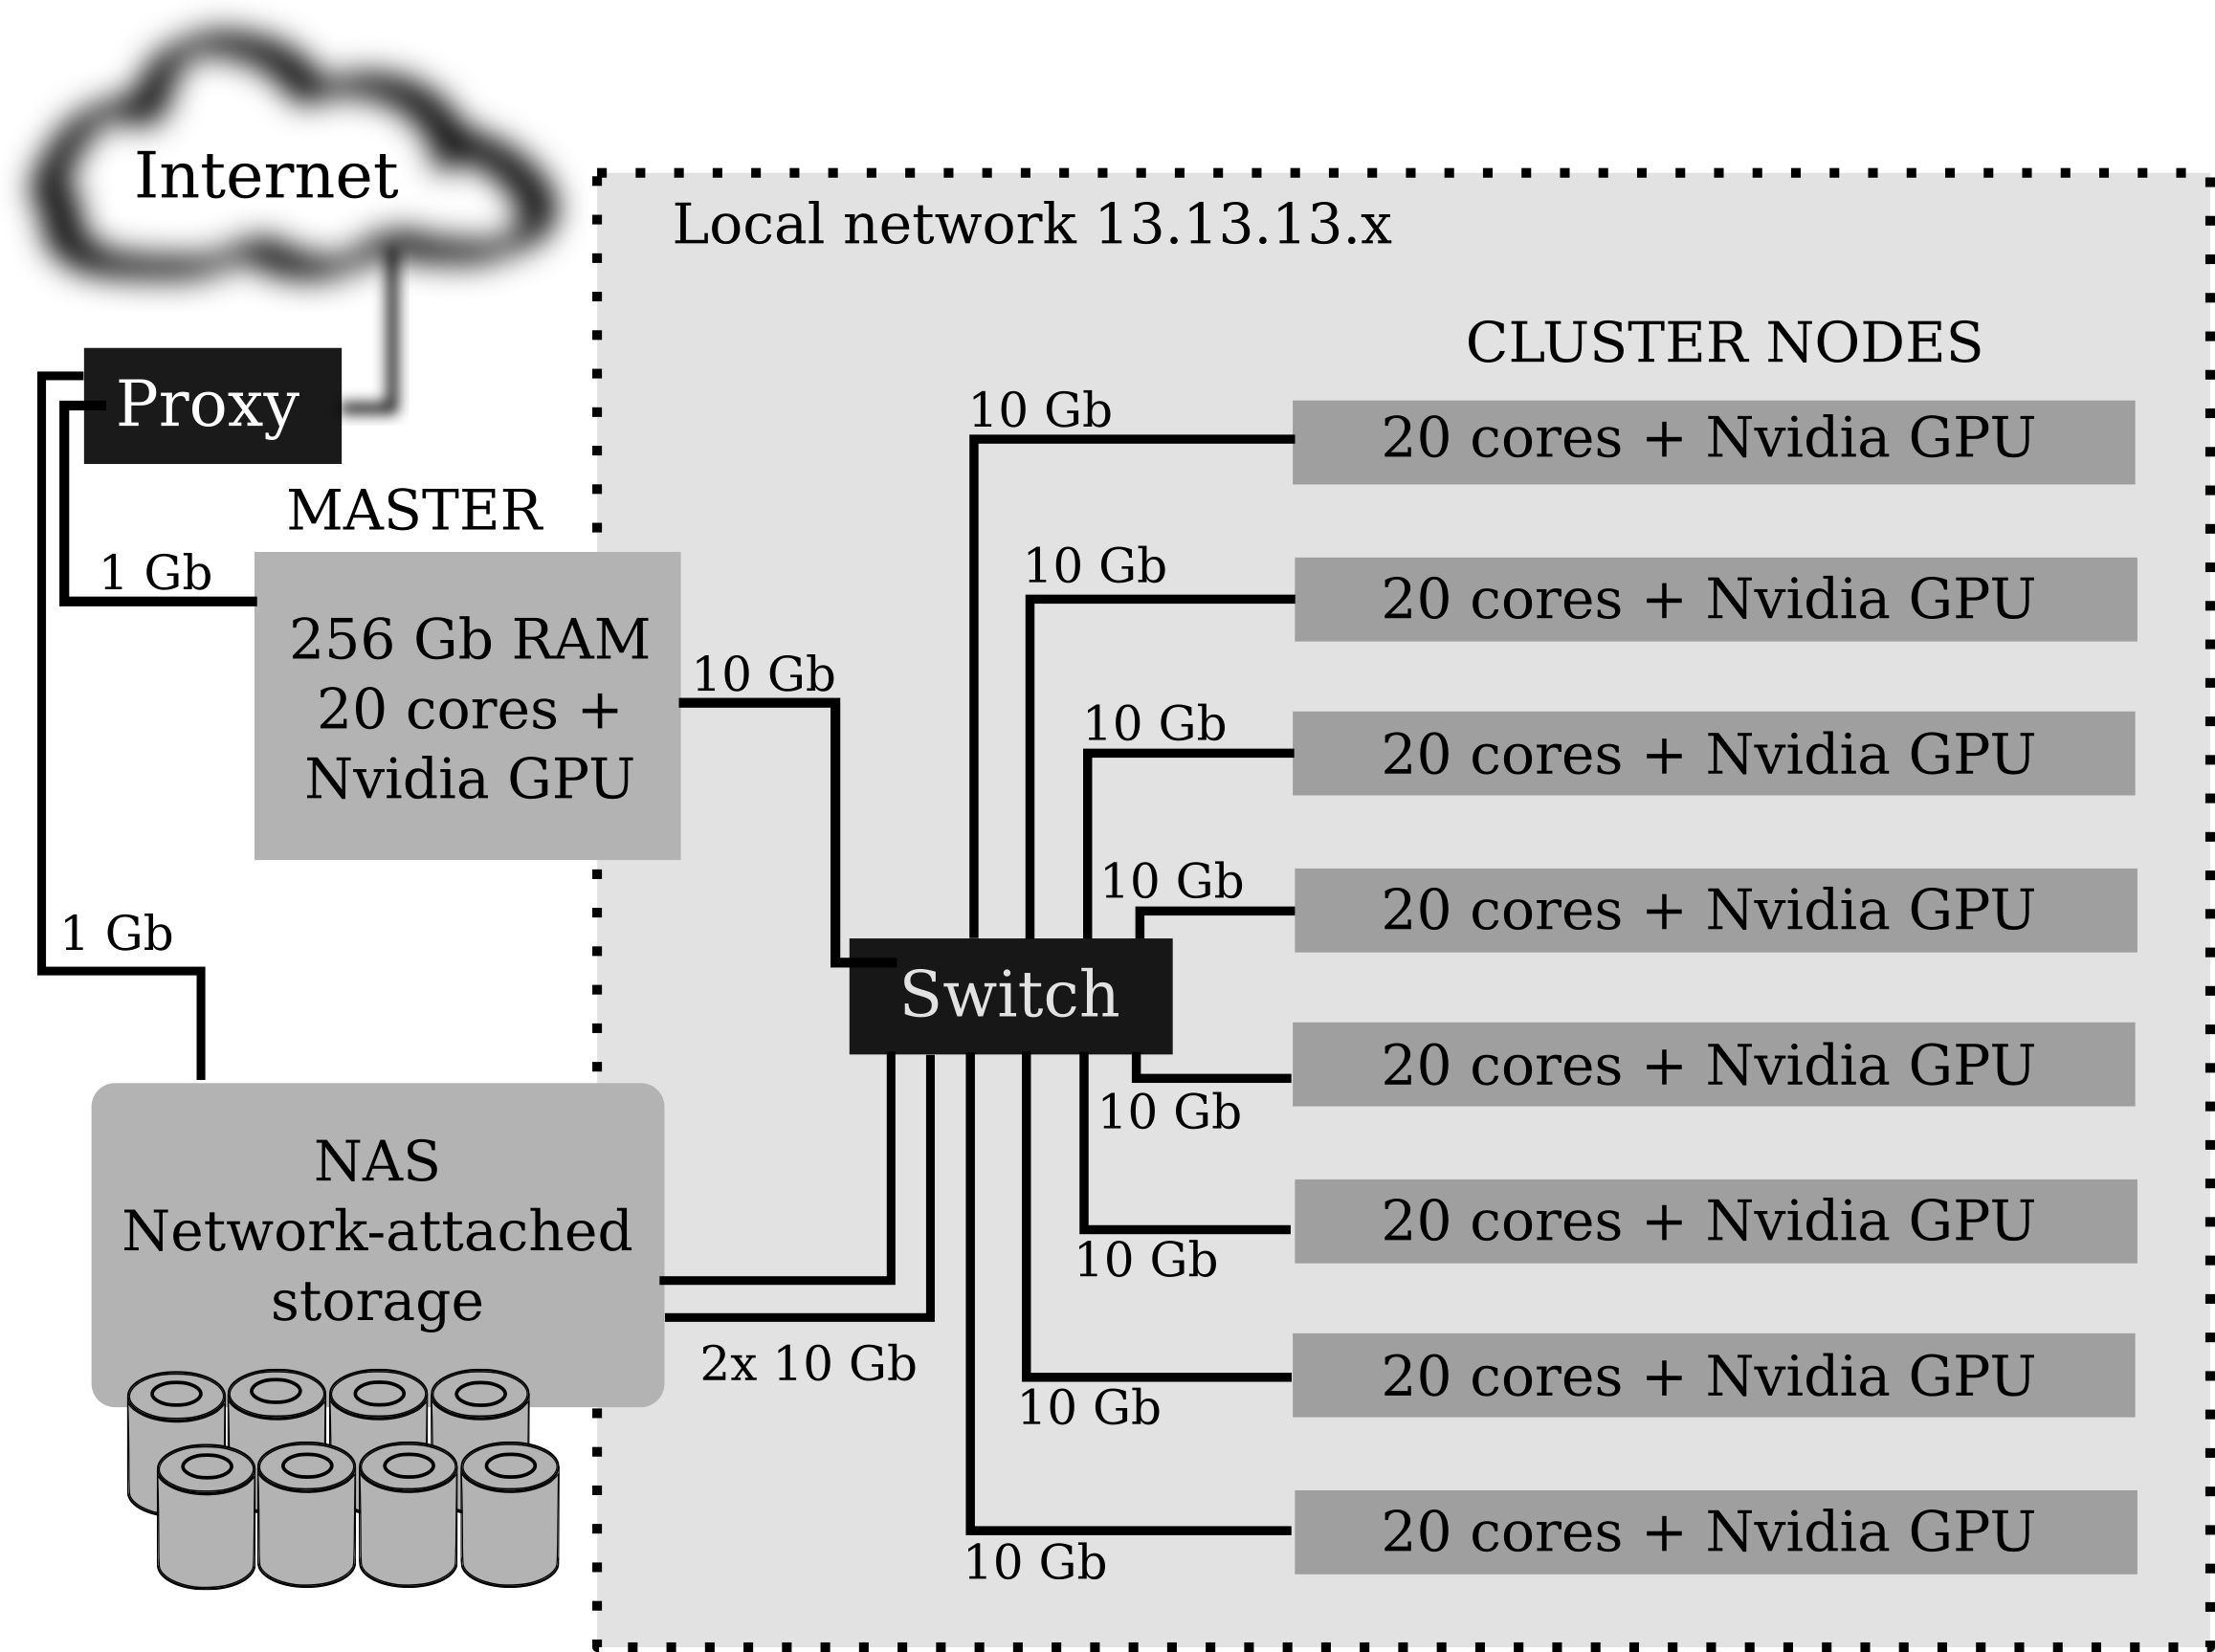
\includegraphics[scale=0.45]{images/cluster-rede.png}
  \end{center}
  
%  \begin{tikzpicture}[remember picture,overlay]
%    \node[anchor=center, inner sep=0] (img1) at (0,0) {\includegraphics[scale=0.2]{images/duas.jpg}};
%    \begin{scope}[
%        x={(img1.south east)},
%        y={(img1.north west)}
%      ]
%      \node [red, font=\bfseries] at (0.25,0.65) {$P(X|Y)$};
%    \end{scope}
%  \end{tikzpicture}
\end{frame}



%-------------------------------------------------
%{\setbeamercolor{background canvas}{bg=black}
%  \setbeamercolor{frametitle}{fg=red}
%  \setbeamercolor{normal text}{fg=red}
%  \usebeamercolor[fg]{normal text}


\section{Software}
%-------------------------------------------------
%

\subsection{Structural}
%-------------------------------------------------
%\begin{frame}
%  \frametitle{Gluster: what is it? (Attention to the G!)}
%  \framesubtitle{It is a distributed filesystem: \textbf{GlusterFS}}

%\textbullet  \textit{Free and open source software}:\\% exatamente! Gratuito e de código aberto (não que pensemos em modificá-lo...)\\
%\textbullet  Native to the system OS: installing and updating done trought official repository. Garanteed compatibility.
%  \vspace{10px}
%  Some of its features:
%  \begin{enumerate}
%  \item Mirroring;
%  \item Replication;
%  \item \textit{Striping};
%  \item Fault Tolerance;
%  \item Quotas;
%  \end{enumerate}
%  \vspace{10px}
%  Our system makes use of \textbf{replication}, \textbf{fault tolerance} and \textbf{quotas}.
%\end{frame}


%
%-------------------------------------------------
%\begin{frame}[fragile]
%  \frametitle{Acesso à memória compartilhada - Criação}
%  \framesubtitle{Exemplo1}
% \begin{lstlisting}%[caption={Fragmento do código-fonte da criação das estruturas de memória compartilhada.}\label{lst:createshm}]
%   // Three C standard arrays are created to shared data with milonga
%   double *shmTarray = NULL;
%   double *shmQarray = NULL;
% \end{lstlisting}
%\end{frame}


%-------------------------------------------------
\begin{frame}
  \frametitle{Software}
  \framesubtitle{Workload Manager \textit{Slurm}}
%  \textbullet The internals of \textit{slurm} workload system.\\
  \begin{figure}
  \centering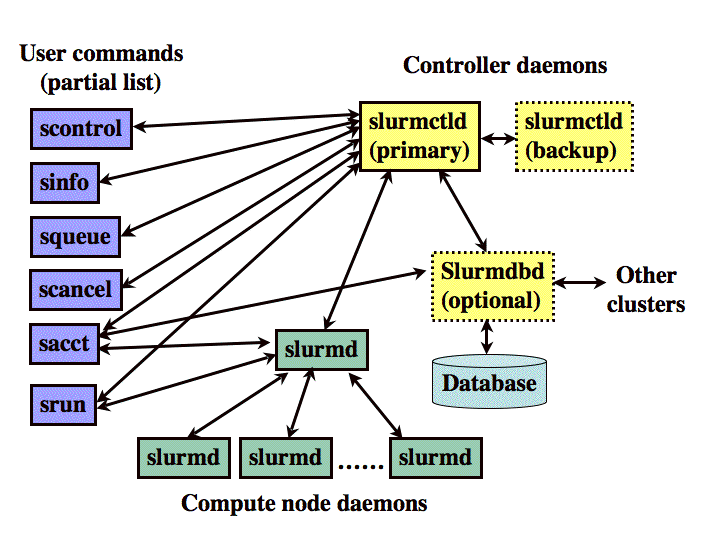
\includegraphics[scale=0.35]{images/slurm-arch.png}
  \caption{Slurm architecture. (Source: Slurm website)}
  \end{figure}
\end{frame}

%-------------------------------------------------
\begin{frame}
  \frametitle{Software}
  \framesubtitle{\textit{Slurm} Report and Queue commands example}
%  \textbullet The internals of \textit{slurm} workload system.\\
%  \begin{figure}
  \centering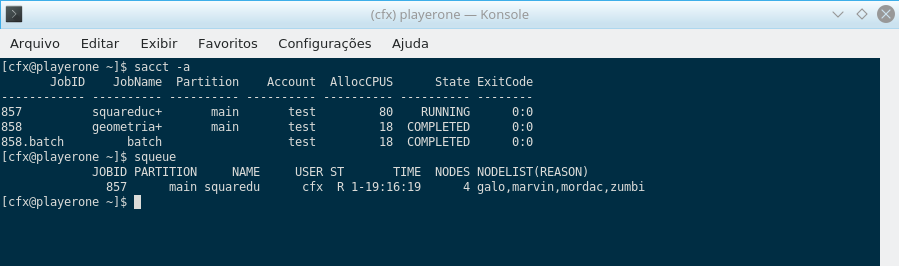
\includegraphics[scale=0.45]{images/Screenshot_20190719_152935.png}
%  \end{figure}
\end{frame}

%-------------------------------------------------
\begin{frame}
  \frametitle{Monitoring System}
  \framesubtitle{Ganglia: detailed node load (\textbf{only six nodes shown})}
  \centering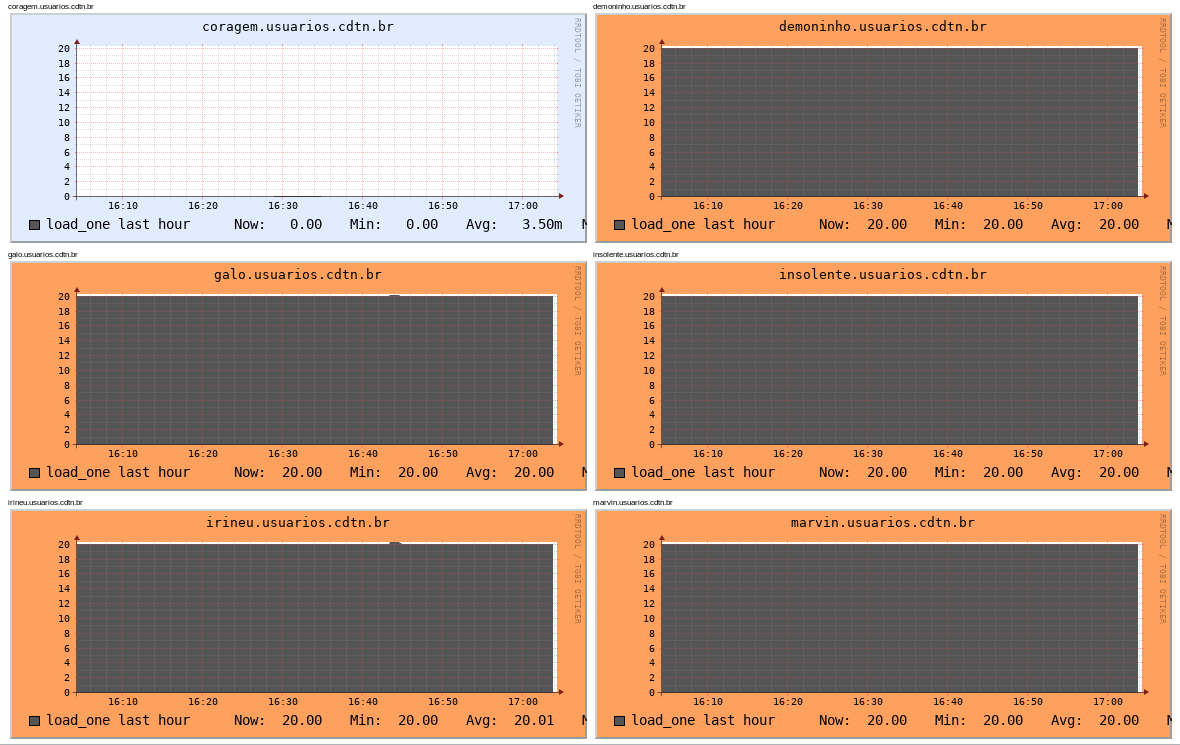
\includegraphics[scale=0.36]{images/ganglia_nodes.png}
\end{frame}


%-------------------------------------------------
\begin{frame}
  \frametitle{Monitoring System}
  \framesubtitle{Ganglia: Overview os system's load}
  \centering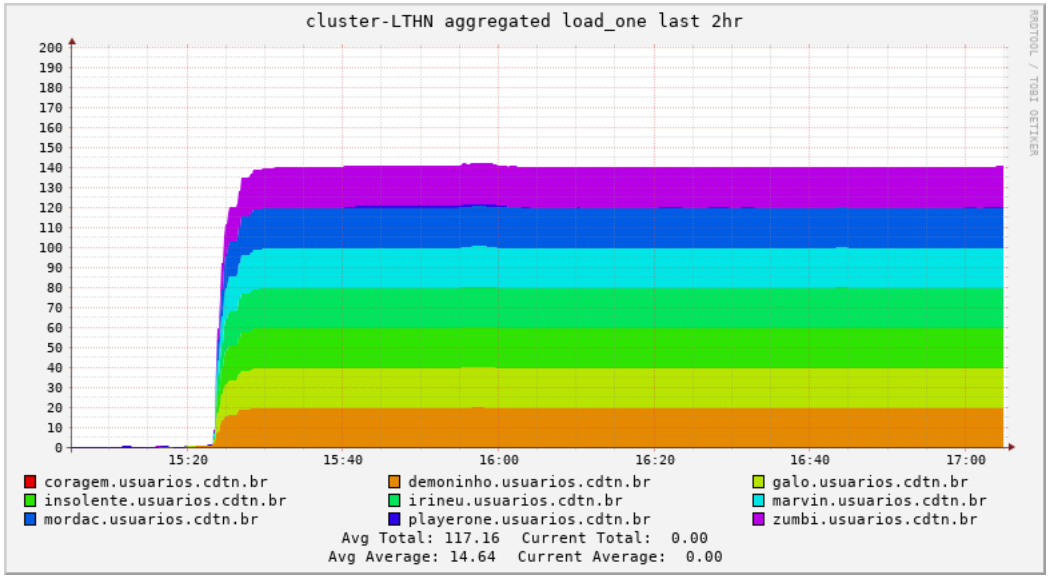
\includegraphics[scale=0.40]{images/ganglia_rainbow.png}
\end{frame}


%-------------------------------------------------
\subsection{Applications}
\begin{frame}
  \frametitle{Software}
  \framesubtitle{What do we have currently available?}
%\centering
  \begin{itemize}
  \item \textbf{Serpent2 Monte Carlo};
  \item \textbf{MCNP 6};
  \item \textbf{OpenFOAM 6};
  \item \textbf{ANSYS package};
  \item \textbf{SCALE 6.2.3};
  \item \textbf{Matlab}.
  \end{itemize}
  \vspace{10px}
  Disk space to accomodate other/new applications. 
\end{frame}

%-------------------------------------------------
\begin{frame}
  \frametitle{Software}
  \framesubtitle{How to use it?}
  A screenshot of the login session.\\
  \vspace{10px}
  \centering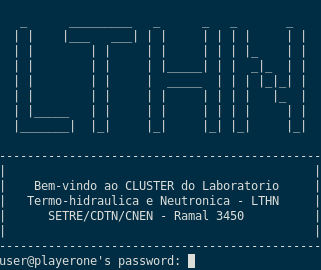
\includegraphics[scale=0.80]{images/p1login.png}
\end{frame}


\section{Conclusions}
%-------------------------------------------------
\begin{frame}
  \frametitle{Conclusions}
  \framesubtitle{General considerations}
  \begin{itemize}
  \item Availability record: 98 days and 12 hours.
  \end{itemize}
\end{frame}

\subsection{Future improvements}
%-------------------------------------------------
\begin{frame}
  \frametitle{Future improvements}
  \framesubtitle{Where we want to be}
  In such kind of system, there is always an enourmous list of possible improvements. We keep the list small as the size of the team that manages the system.
  \vspace{10px}
  Small, but not empty:
  \vspace{10px}
  \begin{itemize}
  \item Use of GPU/accelerators for remote visualization (VirtualGL);
  \item Improvement of measures to allow 'real' 24/7 availability, such as air-conditioning system and no-break connected to an existent diesel generator;
  \item Control and automatic response to events such abrupt change in room's temperature and on-line monitoring of power supply.
  \end{itemize}
  
\end{frame}

%-------------------------------------------------
\begin{frame}
 \vfill
  \begin{beamercolorbox}[center]{title}
     \Huge{Thank you!}
  \end{beamercolorbox}
  \vfill

\end{frame}

%-------------------------------------------------
%\begin{frame}[allowframebreaks]
%        \frametitle{Referências}
%        \bibliographystyle{amsalpha}
%        \bibliography{apre.bib}
%\end{frame}


%-------------------------------------------------
% Frame escondido
%\begin{frame}[noframenumbering]
%  \frametitle{Respostas}
%  \framesubtitle{Seções de choque}
%  Tratamento complexo.
%\end{frame}


\end{document}

